% Original book diagram: fig:explore_exploit
% Book source: sections/Part_V/motion_planning.tex
% Original diagram authorship retained. Visual design: Ziad Mosalam.
\documentclass[11pt,border=8pt]{standalone}
\usepackage{amsmath,amssymb,graphicx,tikz}
\usetikzlibrary{arrows.meta,automata,positioning,calc,shapes.geometric,fit,backgrounds,patterns}
\newcommand{\vect}[1]{\mathbf{#1}}
\newcommand{\mat}[1]{\mathbf{#1}}
\newcommand{\Normal}{\mathcal{N}}
\newcommand{\prob}{p}
\newcommand{\E}{\mathbb{E}}
\newcommand{\Var}{\mathrm{Var}}
\newcommand{\Cov}{\mathrm{Cov}}
\newcommand{\CovP}{\mathbf{P}}
\newcommand{\Prob}{\mathbb{P}}
\setlength{\textwidth}{6.5in}
% Shared visual vocabulary for the book's original diagrams.
% Figures opt in explicitly, so unrelated text and existing additions are unchanged.
\definecolor{BookBlue}{HTML}{003262}
\definecolor{BookGold}{HTML}{B17A00}
\definecolor{BookTeal}{HTML}{247C86}
\definecolor{BookInk}{HTML}{30363B}
\definecolor{BookLight}{HTML}{E9EFF5}
\tikzset{
  book figure/.style={font=\small\rmfamily, color=BookBlue, text=BookInk,
    line width=0.8pt, >=Latex},
  book axis/.style={->, draw=BookInk, line width=0.6pt},
  book link/.style={->, draw=BookBlue, line width=0.8pt},
  book observation/.style={draw=BookGold, fill=BookGold!8},
  book state/.style={draw=BookBlue, fill=BookLight},
  book note/.style={font=\footnotesize\rmfamily, text=BookInk}
}

\begin{document}
% Requires: \usepackage{tikz} \usetikzlibrary{arrows.meta}
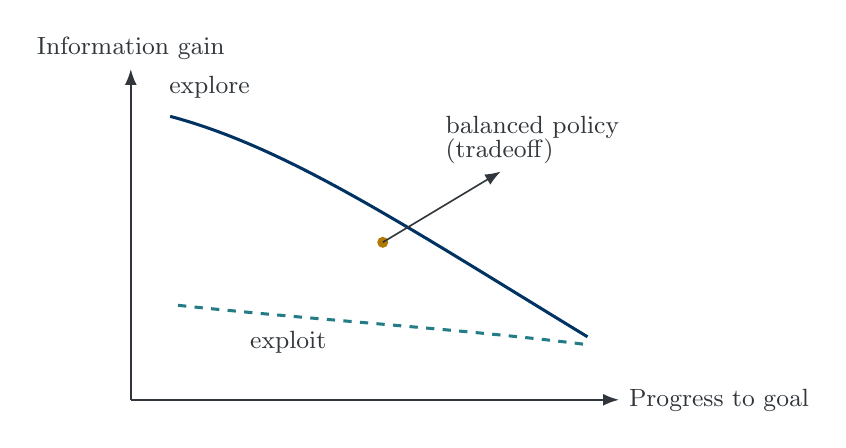
\begin{tikzpicture}[book figure, >=Latex, scale=1.0]
  \draw[book axis] (0,0) -- (6.2,0) node[right] {Progress to goal};
  \draw[book axis] (0,0) -- (0,4.2) node[above] {Information gain};

  % Curves (schematic)
  \draw[BookBlue,line width=1.1pt] (0.5,3.6) .. controls (2.0,3.2) and (3.5,2.2) .. (5.8,0.8);
  \node[above] at (1.0,3.7) {\small explore};

  \draw[BookTeal,line width=1.1pt,dashed] (0.6,1.2) .. controls (2.5,1.0) and (4.2,0.9) .. (5.8,0.7);
  \node[below] at (2.0,1.0) {\small exploit};

  % Sweet spot
  \fill[BookGold] (3.2,2.0) circle (2pt);
  \draw[book axis] (3.2,2.0) -- (4.7,2.9);
  \node[align=left] at (5.1,3.3) {\small balanced policy\\[-2pt]
  \small (tradeoff)};
\end{tikzpicture}
\end{document}
